\chapter{Materialien und Methode} \label{ch:database}

\section{Aufbau der \acs{db}} \label{sec:dbdevelop}

Für die Durchführung dieses Projekts wurde ein relationales \ac{db} Schema in PostgreSQL entwickelt. Die Nutzung von PostgreSQL in diesem Projekt basiert sich darauf, dass dies ein weitverbreitetes \ac{rdbms} im \ac{miracum} Konsortium ist. Andererseits ist PostgreSQL ein freies Open Source \ac{rdbms} mit vielen Features \cite{postgres}.

Für die Implementierung der \ac{db} wurden die \ac{sql}-Anweisungen, nach Empfehlung in der Liesmich-Dateie der Fassungen, angepasst \cite{readmel}. Außerhalb von den vorher genannten Anpassungen wurde die Tabelle \glqq\textsf{kodes}\grqq{} auch erweitert und modifiziert. In dieser Tabelle wurde die Spalte \glqq\textsf{ver}\grqq{} für die Speicherung der Auffassungen oder Versionen eingefügt und die Spalte \textsf{fünfsteller} wurde zu \glqq\textsf{fuenfsteller}\grqq{} umbenannt, um Probleme mit Zeichen-Kodierung zu verhindern. Diese Veränderungen sind schwarz in der Tabelle \glqq\textsf{kodes}\grqq{} der Abbildung~\ref{fig:reldb2} gekennzeichnet. Noch dazu wurden drei neuen Tabellen eingefügt, um die Veröffentlichung Daten (\glqq\textsf{icd10gm\_release\_info}\grqq{}), Speicherung (\glqq\textsf{icd10gm}\grqq{}) und Historisierung \glqq\textsf{icd10gm\_history}\grqq{} aller verfügbaren \ac{icd10gm} von 2007 bis 2021 zu steuern. Solche Tabellen sind mit gelben Kopfzeilen in der Abbildung~\ref{fig:reldb2} repräsentiert.

\section{Funktion der Tabellen} \label{sec:functab}

\section{Tabelle \glqq\textsf{kodes}\grqq{} von \acs{bfarm}} \label{subsec:bfarmtables}

Die Tabellen von \glqq\textsf{kodes}\grqq{} vom \ac{bfarm}-Schema beinhalten die Information der \ac{csv}-Dateien von nur einer Fassung und enthält damit die Anfangsdaten für die Tabellen \glqq\textsf{icd10gm}\grqq{} und \glqq\textsf{icd10gm\_history}\grqq{}.

\clearpage	

\begin{figure}[ht]
	\centering
	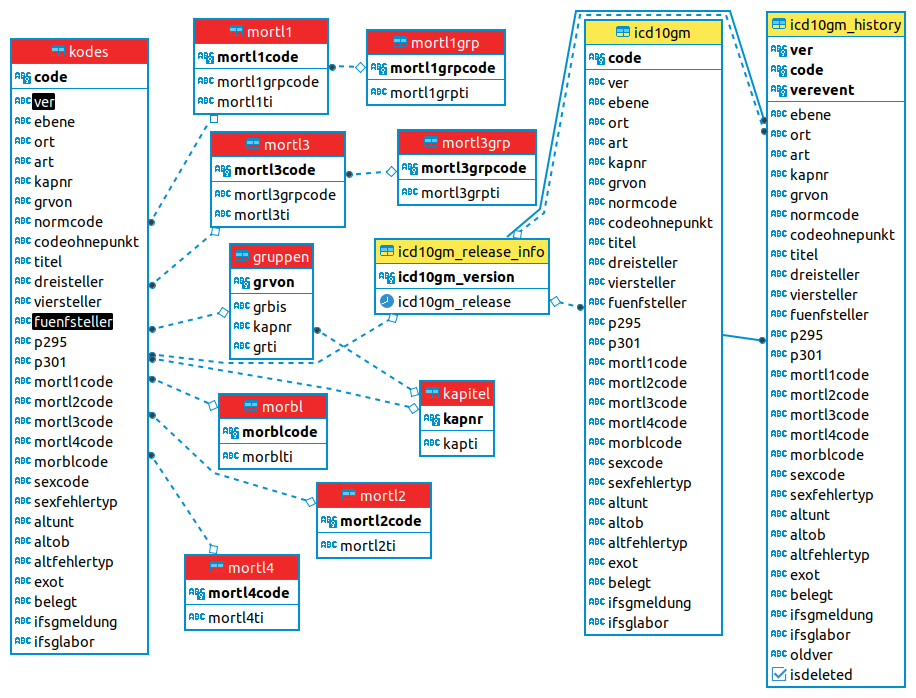
\includegraphics[height=10cm]{figures/icdSqlSchema}
	\caption[Datenbankstruktur]{Datenbankstruktur für die Steuerung der \ac{icd10gm}. Die Tabellen von \ac{bfarm} sind mit Kopfzeilen in rot gekennzeichnet, die Spalten in schwarz in diesen Tabellen sind die vorgenommenen Erweiterungen und Modifikationen. Die Tabellen mit Kopfzeilen in gelb sind die neuen eingeführten Tabellen für die Historisierung der \ac{icd10gm}.}
	\label{fig:reldb2}
\end{figure}

\subsection{Neuen Tabellen} \label{subsec:newtables}

Für die Erfassung der Datierung der Veröffentlichungen der Versionen wurde die Tabelle \glqq\textsf{icd10gm\_release\_info}\grqq{} erstellt. Diese speichert den Identifikator oder das Jahr der Version in der Spalte \glqq\textsf{icd10gm\_version}\grqq{} als Hauptschlüssel und das Datum der Veröffentlichung in der Spalte \glqq\textsf{icd10gm\_release}\grqq{}. Diese hat das Format \glqq\textsf{JJJJ-MM-TT}\grqq{}. Wobei \glqq J\grqq{} das Jahr, \glqq M\grqq{} der Monat und \glqq T\grqq{} der Tag darstellen.

Die \ac{icd10gm} von 2007 bis 2021, werden in der Tabelle \glqq\textsf{icd10gm}\grqq{} gespeichert. In dieser Tabelle wird die Information der noch gültigen \ac{icd10gm} aktualisiert. Die gelöschten \ac{icd10gm} beinhalten die Information der letzten Aktualisierung. Die Spalte \textsf{code}\grqq{} dieser Tabelle ist der Hauptschlüssel, genau wie in der Tabelle \glqq\textsf{kodes}\grqq{} vom \ac{bfarm}-Schema. \glqq\textsf{ver}\grqq{} speichert den Identifikator der Version der Insertion oder der letzten Änderung und ist ein Fremdschlüssel, der zu der Spalte \glqq\textsf{icd10gm\_version}\grqq{} der Tabelle \glqq\textsf{icd10gm\_release\_info}\grqq{} zeigt.

Die Tabelle \glqq\textsf{icd10gm\_history}\grqq{} enthält die Information der \ac{icd10gm}, die im Laufe der Zeit eingefügt, gelöscht oder geändert wurden. Die Besonderheiten diese Tabelle sind die Spalten \glqq\textsf{ver}\grqq{}, \glqq\textsf{oldver}\grqq{}, \glqq\textsf{verevent}\grqq{} und \glqq\textsf{isdeleted}\grqq{}. Die Identifikatoren vergangener Versionen einer \ac{icd10gm} werden in der Spalte \glqq\textsf{oldver}\grqq{} gespeichert. Die Spalte \glqq\textsf{ver}\grqq{} enthält den Identifikator der Fassungen bei deren eine \ac{icd10gm} eingefügt, gelöscht oder modifiziert wurde. Die Ereignisse einer Insertion, Änderung, Löschung oder Wiederverwendung werden mit den Buchstaben \glqq\textsf{I}\grqq{} (insert), \glqq\textsf{U}\grqq{} (update), \glqq\textsf{D}\grqq{} (delete) und \glqq\textsf{DI}\grqq{} (delete insert) in der Spalte \glqq\textsf{verevent}\grqq{} kodiert und gespeichert. Da manche Schlüsselnummern wieder benutzt wurden, wird die Spalte \textsf{isdeleted} mit dem Wert \glqq true\grqq{} markiert, wenn ein \ac{icd10gm} gelöscht wird. Diese Spalte wird auf \glqq false\grqq{} bei einer Wiederverwendung gesetzt.

\section{Fluss der Information} \label{sec:dbrun}

Mit Hilfe einer \ac{etl}-Strecke werden die Daten aus der \ac{zip}-Datei in der \ac{db} importiert. Die Information der Veröffentlichung der \ac{icd10gm} wird in der Tabelle \glqq\textsf{icd10gm\_release \_info}\grqq{} eingefügt. Bei jeder Ladung wird die Information der Tabelle \glqq\textsf{kodes}\grqq{} vorher gelöscht und mit neuen Datensätzen geladen. 

Die Kodes, die vorher nicht in der Tabelle \glqq\textsf{icd10gm}\grqq{} vorhanden waren, werden in dieser und in der Tabelle \glqq\textsf{icd10gm\_history}\grqq{} kopiert. Diese Datensätze werden in \glqq\textsf{icd10gm\_history}\grqq{} als eingefügt markiert. 

Nicht in \glqq\textsf{kodes}\grqq{} existierende \ac{icd10gm} werden aus \glqq\textsf{icd10gm}\grqq{} in \glqq\textsf{icd10gm\_history}\grqq{} kopiert. Diese Kopie wird als gelöscht markiert, und enthält die Indikatoren der Fassung der Insertion oder der letzten Änderung in der Spalte \textsf{oldver}\grqq{}, und der Fassung der Löschung in der Spalte \glqq\textsf{ver}\grqq{}. 

Existierende Kodierungen mit modifizierten Informationen werden in der Tabelle \glqq\textsf{icd10gm}\grqq{} aktualisiert und nachher in \glqq\textsf{icd10gm\_history}\grqq{} hinzugefügt.In diesem Fall werden auch die Indikatoren der alten und neuen Fassung registriert und der Datensatz als modifiziert markiert.

Dieser Fluss der Information ist im Datenflussdiagramm der Abbildung~\ref{fig:dbflow} repräsentiert. Der automatisierte Prozessablauf in der \ac{db} ist durch Triggers in den Tabellen \glqq\textsf{kodes}\grqq{} und \glqq\textsf{icd10gm}\grqq{} gesteuert.

\begin{figure}[ht]
	\centering
	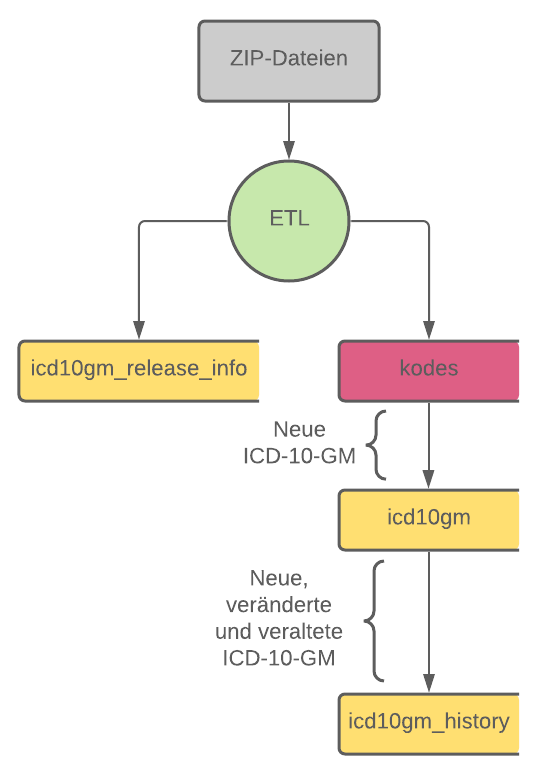
\includegraphics[height=10cm]{figures/dbflow}
	\caption[Datenfluss des Prozesses]{Datenflussdiagramm der Information von den \ac{zip}-Dateien bis zum Import in der \ac{db}.}
	\label{fig:dbflow}
\end{figure} 